\subsection{Some Modified Armstrong--Frederick Evolution Rules}
In the scalar form, the Armstrong--Frederick evolution rule is equivalent to the following ordinary differential equation,
\begin{equation}
    y'=b\left(a-y\right),
\end{equation}
it can be explicitly integrated to give the solution for the initial condition $y(0)=0$,
\begin{equation}
    y(x)=a\left(1-\exp\left(-bx\right)\right),
\end{equation}
which defines a curve that asymptotically approaches the bound $a$.

To employ a non-constant bound, it is possible to simply replace the constant $a$ by a function $f(x)$ in the ODE.
However, as noted in the literature, the corresponding solution is not strictly bounded by $f(x)$.
\figref{fig:examples} presents both hardening and softening examples.
As can be seen from the figure, the solution may overshoot for softening bounds.
\begin{figure}[htb]
\centering\scriptsize
    \begin{subfigure}{0.48\textwidth}\centering
        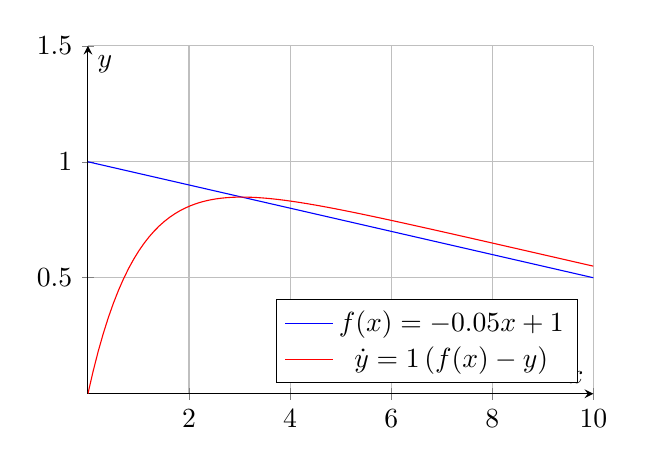
\begin{tikzpicture}
            \begin{axis}[axis lines=middle,xlabel=$x$,ylabel=$y$,grid=both,width=8cm,height=6cm,legend pos=south east,ymin=0,ymax=1.5]
                \pgfmathsetmacro{\aa}{-.05}
                \pgfmathsetmacro{\bb}{1}
                \pgfmathsetmacro{\cc}{1}
                \addplot[domain=0:10,samples=100,color=blue]{\aa*x+\bb};
                \addplot[domain=0:10,samples=100,color=red]{\aa*x+\bb+(\aa/\cc-\bb)*exp(-\cc*x)-\aa/\cc};
                \addlegendentry{$f(x)=\aa{}x+\bb$}
                \addlegendentry{$\dot{y}=\cc\left(f(x)-y\right)$}
            \end{axis}
        \end{tikzpicture}
        \caption{softening}
    \end{subfigure}\hfill
    \begin{subfigure}{0.48\textwidth}\centering
        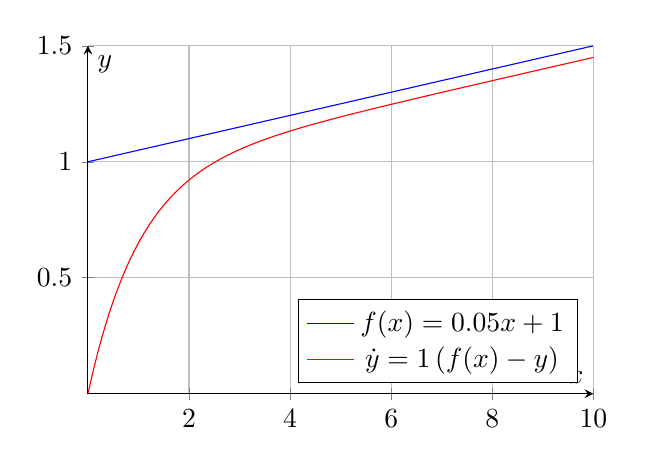
\begin{tikzpicture}
            \begin{axis}[axis lines=middle,xlabel=$x$,ylabel=$y$,grid=both,width=8cm,height=6cm,legend pos=south east,ymin=0,ymax=1.5]
                \pgfmathsetmacro{\aa}{0.05}
                \pgfmathsetmacro{\bb}{1}
                \pgfmathsetmacro{\cc}{1}
                \addplot[domain=0:10,samples=100,color=blue]{\aa*x+\bb};
                \addplot[domain=0:10,samples=100,color=red]{\aa*x+\bb+(\aa/\cc-\bb)*exp(-\cc*x)-\aa/\cc};
                \addlegendentry{$f(x)=\aa{}x+\bb$}
                \addlegendentry{$\dot{y}=\cc\left(f(x)-y\right)$}
            \end{axis}
        \end{tikzpicture}
        \caption{hardening}
    \end{subfigure}
    \caption{examples}\label{fig:examples}
\end{figure}
\subsubsection{A Simple Modification}
To ensure that the solution is bounded by $f(x)$, let's consider the following function,
\begin{gather}
    y=f(x)\left(1-\exp\left(-bx\right)\right),
\end{gather}
since $1-\exp\left(-bx\right)\leqslant1$, it is guaranteed that $y\leqslant{}f(x)$.
The corresponding ODE can be derived as follows,
\begin{gather}\label{eq:strict_bound}
    y'=fb\exp\left(-bx\right)+f'\left(1-\exp\left(-bx\right)\right)=b\left(f-y\right)+\dfrac{f'}{f}y.
\end{gather}
After careful comparison, one could observe that \eqsref{eq:strict_bound} is in fact identical to the evolution rule proposed recently.

Then instead of defining an evolution rule for $\bc$, which turns out to be cumbersome, one can apply the following decomposition,
\begin{gather}
    \bc-\balpha=\sigma^y\bd,
\end{gather}
then the evolution of $\bc$ can be equivalently described by the evolution of $\bd$, which takes a very simple form,
\begin{gather}
    \dot{\bd}=c_e\left(\sqrt{\dfrac{2}{3}}z_e\bn-\bd\right)\gamma.
\end{gather}